%; whizzy chapter -dvi
% -initex iniptex -latex platex -format platex -bibtex jbibtex -fmt fmt
% 以上 whizzytex を使用する場合の設定。

%     Tokyo Debian Meeting resources
%     Copyright (C) 2011 Junichi Uekawa
%     Copyright (C) 2011 Nobuhiro Iwamatsu

%     This program is free software; you can redistribute it and/or modify
%     it under the terms of the GNU General Public License as published by
%     the Free Software Foundation; either version 2 of the License, or
%     (at your option) any later version.

%     This program is distributed in the hope that it will be useful,
%     but WITHOUT ANY WARRANTY; without even the implied warranty of
%     MERCHANTABILITY or FITNESS FOR A PARTICULAR PURPOSE.  See the
%     GNU General Public License for more details.

%     You should have received a copy of the GNU General Public License
%     along with this program; if not, write to the Free Software
%     Foundation, Inc., 51 Franklin St, Fifth Floor, Boston, MA  02110-1301 USA

%  preview (shell-command (concat "evince " (replace-regexp-in-string "tex$" "pdf"(buffer-file-name)) "&"))
% 画像ファイルを処理するためにはebbを利用してboundingboxを作成。
%(shell-command "cd image201201; ebb *.png")

%%ここからヘッダ開始。

\documentclass[mingoth,a4paper]{jsarticle}
\usepackage{monthlyreport}

% 日付を定義する、毎月変わります。
\newcommand{\debmtgyear}{2012}
\newcommand{\debmtgmonth}{12}
\newcommand{\debmtgdate}{15}
% (+ (* (- 2012 2005) 12) 12 -1) started from zero
\newcommand{\debmtgnumber}{95}

\begin{document}

\begin{titlepage}
\thispagestyle{empty}
% タイトルページ:編集必要な部分は最初のマクロに飛ばすこと

\vspace*{-2cm}
第\debmtgnumber{}回 東京エリア Debian 勉強会資料\\
\hspace*{-2cm}

\includegraphics{image2012-natsu/dotdeb.pdf}\\
\hfill{}\debmtgyear{}年\debmtgmonth{}月\debmtgdate{}日

% ここはアップデートすること
% 全角文字にしないとフォントのサイズが合わないので注意
\rotatebox{10}{\fontsize{32}{32} {\gt 特集1: 2012年の振り返り}}

\rotatebox{10}{\fontsize{32}{32} {\gt 特集2: 著作権法改正}}

\vspace*{-2cm}
\hfill{}
\includegraphics[height=6cm]{image200502/openlogo-nd.eps}
\end{titlepage}

\dancersection{Introduction}{上川 純一}

\begin{multicols}{2}
 

 今月のDebian勉強会へようこそ。これからDebianの世界にあしを踏み入れると
 いう方も、すでにどっぷりとつかっているという方も、月に一回Debianについ
 て語りませんか?

 Debian勉強会の目的は下記です。

 \begin{itemize}
 \item \underline{Debian Developer} (開発者)の育成。
 \item 日本語での「\underline{開発に関する情報}」を整理してまとめ、アップデートする。
 \item \underline{場}の提供。
 \begin{itemize}
  \item 普段ばらばらな場所にいる人々が face-to-face で出会える場を提供
	する。
  \item Debian のためになることを語る場を提供する。
  \item Debianについて語る場を提供する。
 \end{itemize}
 \end{itemize}		

 Debianの勉強会ということで究極的には参加者全員がDebian Packageをがりがり
 と作るスーパーハッカーになった姿を妄想しています。情報の共有・活用を通し
 て Debianの今後の能動的な展開への土台として、「場」としての空間を提供す
 るのが目的です。

\end{multicols}

\newpage

\begin{minipage}[b]{0.2\hsize}
 \definecolor{titleback}{gray}{0.9}
 \colorbox{titleback}{\rotatebox{90}{\fontsize{80}{80} {\gt デビアン勉強会} }}
\end{minipage}
\begin{minipage}[b]{0.8\hsize}
\hrule
\vspace{2mm}
\hrule
\begin{multicols}{2}
\tableofcontents
\end{multicols}
\vspace{2mm}
\hrule
\end{minipage}

\dancersection{事前課題}{上川 純一}

今回の事前課題は以下です:
\begin{enumerate}
 \item 2012年の勉強会のテーマとして各月なにをするべきか提案してくさい。 
 \item 自分がどのテーマを担当したいか提案してください。
\end{enumerate}
この課題に対して提出いただいた内容は以下です。
\begin{multicols}{2}
{\small
 %; whizzy-master ../debianmeetingresume201212.tex
% $B0J>e$N@_Dj$r$7$F$$$k$?$a!"$3$N%U%!%$%k$G(B M-x whizzytex $B$9$k$H!"(B
% whizzytex$B$,MxMQ$G$-$^$9(B

\begin{prework}{ $B5HLn(B(yy\_y\_ja\_jp) }

\preworksection{DFSG$B$K$*$$$F$N<+M3$K$D$$$FO@$8$F$/$@$5$$!#(B}

 $B<+M3$r<i$k$?$a$N@)8B$G$"$k!#(B

\preworksection{Debian$B$K4X$7$F!"#2#0#1#2G/$r$U$j$+$($C$F#2#0#1#3G/$d$C$F$*$-$?$$$3$H$rO@$8$F$/$@$5$$!#(B}

 Bug squashing$B!$(BDDTP$B$J$I$G$NK]Lu(B
\end{prework}

\begin{prework}{ seiji-n }
\preworksection{DFSG$B$K$*$$$F$N<+M3$K$D$$$FO@$8$F$/$@$5$$!#(B}

5.$B$9$Y$F$N8D?M!"CDBN$NJ?Ey(B

6.$B%i%$%;%s%9$O!"$9$Y$F$N8D?M$dCDBN$r:9JL$7$F$O$J$j$^$;$s!#(B

DFSG$B$N>e5-3F>r9`$K4X$7$F!"%F%m%j%9%HEyH?<R2qCDBN$dHH:a<T!"HH:a=8CD$K$h$k(B
$BH?<R2qE*3hF0!"HH:a9T0Y$X$NMxMQ$KBP$7$F!":9JL$G$O$J$/$H6hJL$O$7$F$*$j!"(B
($B5,@)$O$G$-$J$$$J$,$i$b(B)$B7h$7$FA4LLE*$K>5G'$7$F$$$kLu$G$O$J$$$H$$$&(B
$B0U;VI=L@E*$J;v$r$9$Y$-$G$O$J$$$+!#$J$<$7$J$$$N$+!#$=$N>e$G$N<+M3$G$O(B
$B$J$$$+$H9M$($F$$$^$9!#(B


$BL\I8J,Ln$NJ?Ey(B

\preworksection{Debian$B$K4X$7$F!"#2#0#1#2G/$r$U$j$+$($C$F#2#0#1#3G/$d$C$F$*$-$?$$$3$H$rO@$8$F$/$@$5$$!#(B}

$B62=L$G$9$,(B2012$BG/$O(BDebian$B$K4X$7$F2?$b$7$F$$$^$;$s!#$3$l$+$i3X$s$G9T$-$?$$$H;W$$$^$9!#(B

\end{prework}

\begin{prework}{ dictoss($B?yK\!!E5=<(B) }

\preworksection{DFSG$B$K$*$$$F$N<+M3$K$D$$$FO@$8$F$/$@$5$$!#(B}

$B#9HVL\$N!V%i%$%;%s%9$OB>$N%=%U%H%&%'%"$r?/32$7$J$$!W$H$"$k!#(BLGPL$B%i%$%;%s%9$O(BGFSG$B8_49%i%$%;%s%9$@$,<B9T;~$OB>$N%=%U%H%&%'%"$N<+M3$r?/32$7$F$k>l9g$,$"$j$=$&$J5$$,$9$k$,$I$&$J$s$@$m$&$+!#(B


\preworksection{Debian$B$K4X$7$F!"#2#0#1#2G/$r$U$j$+$($C$F#2#0#1#3G/$d$C$F$*$-$?$$$3$H$rO@$8$F$/$@$5$$!#(B}

$B:#G/$O(Barmel$B%"!<%-%F%/%A%c$N(Bdebian$B$r=i$a$F<+J,$G%$%s%9%H!<%k$7$F$_$?!#@h?MC#$NCN7C$,$"$k$?$a3d$H$9$s$J$jF~$C$F$7$^$C$F(Bdebian$B$O$9$4$$$H;W$C$?!#MhG/$O(Bmips$B7O$N%O!<%I$rC5$7$F(Bdebian$B$rF~$l$F?'!9;n$7$F$_$?$$$H;W$$$^$9!#(B
\end{prework}

\begin{prework}{ $B%-%?%O%i(B }
\preworksection{DFSG$B$K$*$$$F$N<+M3$K$D$$$FO@$8$F$/$@$5$$!#(B}

 $BO@$8$kDx$NCNG=$O$J$$$N$G!"BX$o$j$K46A[$r!#(B
$BB>$N%i%$%;%s%9Ey$KHf$Y!"4V8}$,9-$/!"8=<BE*$G!"@)8B$,>/$J$/!"(B
$B3+H/<T$N$_$J$i$:MxMQ<T$K$b?4CO$N$h$$<+M3$G$"$k$H;W$&!#(B

\preworksection{Debian$B$K4X$7$F!"#2#0#1#2G/$r$U$j$+$($C$F#2#0#1#3G/$d$C$F$*$-$?$$$3$H$rO@$8$F$/$@$5$$!#(B}
 $B;d;v$G$9$,!"0[F0$G;H$($J$/$J$C$?(BDebian$B<RFb%5!<%P$NBe$o$j$r2?$H$+$7$?$$$G$9$M!#(B
\end{prework}

\begin{prework}{ $B@P0f0lIW(B }

\preworksection{DFSG$B$K$*$$$F$N<+M3$K$D$$$FO@$8$F$/$@$5$$!#(B}

$B$h$/$o$+$j$^$;$s$,!"%=!<%9%3!<%I$N8x3+$H$=$N1?MQ$N<+M3$O0];}$7$F$[$7$$$G$9!#(B

\preworksection{Debian$B$K4X$7$F!"#2#0#1#2G/$r$U$j$+$($C$F#2#0#1#3G/$d$C$F$*$-$?$$$3$H$rO@$8$F$/$@$5$$!#(B}

$B%S%C%0%G!<%?4X78$,!"<g@o>l$K$J$C$F$$$^$9!#(BZFS$B$NE,MQ!"%;%-%e%j%F%#$N6/2=$NLL$+$i!"(BkfreeBSD$B$KCmL\$7$F$$$^$9!#(B2013$BG/$O!"%S%C%0%G!<%?$H(BkfreeBSD$B$G$J$K$+9W8%$,$G$-$l$P$H9M$($F$$$^$9!#(B
\end{prework}

\begin{prework}{ akikazu.sudou }

\preworksection{DFSG$B$K$*$$$F$N<+M3$K$D$$$FO@$8$F$/$@$5$$!#(B}

$B$h$/CN$i$J$$$1$l$I!"(BDFSG$B$N$*$+$2$G:#$N(Bdebian$B$,;H$($k$N$J$i!"$"$j$,$?$$$b$N$@$H;W$$$^$9!#(B

\preworksection{Debian$B$K4X$7$F!"#2#0#1#2G/$r$U$j$+$($C$F#2#0#1#3G/$d$C$F$*$-$?$$$3$H$rO@$8$F$/$@$5$$!#(B}
debian$B%[%9%H$N2>A[4D6-$r$$$8$C$F$_$?$$$G$9!#(B

\end{prework}

\begin{prework}{ $B$J$+$*$1$$$9$1(B }
\preworksection{DFSG$B$K$*$$$F$N<+M3$K$D$$$FO@$8$F$/$@$5$$!#(B}

$B!!(BDebian$B$O!"(BDebian$B<R2q7@Ls$K$h$j!"(BDebian$B%7%9%F%`$H$=$N9=@.MWAG$,(B100\%$B%U(B
 $B%j!<%=%U%H%&%'%"$G$J$1$l$P$J$i$J$$$H5,Dj$7$F$$$^$9!#$=$NCx:nJ*$,!V%U%j!<!W(B
 $B$G$"$k$HH=CG$9$k$?$a$N4p=`$,(BDFSG$B$G$9!#$9$J$o$A!"(BDebian$B$K4^$^$l$k%=%U%H(B
 $B%&%'%"$O!":FG[I[$9$k<+M3!"8D?M$dCDBN!"L\E*$K$h$i$:;HMQ$9$k<+M3!"$*$h$S(B
 $B2~JQ$9$k<+M3$r%f!<%6!<$KM?$($k$b$N$G$J$1$l$P$J$j$^$;$s!#(B

$B!!FC$KL\E*G!2?$KLd$o$:%=%U%H%&%'%"$r;HMQ$9$k<+M3$H!"%=!<%9%3!<%I$rF~<j$7!"(B
 $B$+$D2~JQ$9$k<+M3$O!"3+H/85$,%5%]!<%H$r$d$a$?$H$7$F$b!"!J$d$m$&$H;W$($P!K(B
 $B%f!<%6$,<+J,$?$A$G$J$s$H$+$G$-$k$H$$$&$3$H$G$9!#$3$l$OD94|4V%7%9%F%`$r(B
 $B0];}$9$k$3$H$r5a$a$i$l$k8=>l$K$*$$$FHs>o$K6/NO$JIp4o$K$J$j$^$9!#(B

\end{prework}

\begin{prework}{ $BLnEg!!5.1Q(B }

\preworksection{DFSG$B$K$*$$$F$N<+M3$K$D$$$FO@$8$F$/$@$5$$!#(B}
 debian$B$r<g$K;H$C$F$k$H!"$J$s$+$b$&6u5$$N$h$&$JEv$?$jA0$NB8:_$K46$8$F$7(B
 $B$^$&(BDFSG$B$G$9!#$3$3$G$&$?$o$l$F$$$k<+M3$O!"%(%s%8%K%"%i%$%U$K$H$C$F:GDc(B
 $B8BIT2D7g$J<+M3$@$H8D?ME*$K$O;W$C$F$^$9!#$?$@!"<+J,$NCN8+$,B-$i$J$$0Y$+!"(B
 $B<B$O(BDFSG$B$G$&$?$o$l$F$$$k<+M3$,$I$s$J;v$r5>@7$K$7$F!"$I$s$JEXNO$G$5$5$((B
 $B$i$l$F$$$k$N$+$,$"$^$j$h$/2r$C$F$*$i$:(B...$B$3$N$"$?$jC/$+65$($F!<$C!#(B

\preworksection{Debian$B$K4X$7$F!"#2#0#1#2G/$r$U$j$+$($C$F#2#0#1#3G/$d$C$F$*$-$?$$$3$H$rO@$8$F$/$@$5$$!#(B}

 2012$BG/$O!"$*$+$2$5$^$G!"$A$g$C$H$O%"%&%H%W%C%H$G$-$?!)(B2013$BG/$O$5$i$K%"%&%H%W%C%H!J%O%C%/Ey!K$KNe$_$^$&$9!#(B
\end{prework}

\begin{prework}{ koedoyoshida }

\preworksection{DFSG$B$K$*$$$F$N<+M3$K$D$$$FO@$8$F$/$@$5$$!#(B}

$B%=%U%H%&%'%"3+H/<T$N$?$a$N<+M3$G$9$M!#(B
$B$"$k0UL#6KKL$N%G%#%9%H%j%S%e!<%7%g%s$G$"$j!"(BDebian$B$N:GBg$NFCD'$@$H$*$b$$$^$9!#(B
Ubuntu$B$H$N:GBg$N0c$$$H$$$C$F$bNI$$$N$G$O$J$$$G$7$g$&$+!#(B

\preworksection{Debian$B$K4X$7$F!"#2#0#1#2G/$r$U$j$+$($C$F#2#0#1#3G/$d$C$F$*$-$?$$$3$H$rO@$8$F$/$@$5$$!#(B}

DebianJP$B;22C!#(B
\end{prework}

\begin{prework}{ yamamoto }
\preworksection{DFSG$B$K$*$$$F$N<+M3$K$D$$$FO@$8$F$/$@$5$$!#(B}

DFSG $B$O!"%=%U%H%&%'%"$N<+M3$r3NJ]$9$k$?$a$K$O!"$J$+$J$+$h$/$G$-$?%,%$%I(B
 $B%i%$%s$@$H;W$$$^$9!#$3$l$K$$$/$D$+$N;v9`$r2C$($F(B OSD $B$H$7$?$N$bG<F@$G$-(B
 $B$^$9!#$^$?!"40A4$K%\%i%s%F%#%"%Y!<%9$G$"$k(B Debian $B$K$O!"(B ``$B%U%j!<%=%U%H(B
 $B%&%'%"%3%_%e%K%F%#$H$N!V<R2q7@Ls!W(B'' $B$H6&$K!"(BDebian $B$,M}A[$H$9$k$"$jJ}$rL@<($7!"$3$l$i$K;?F1$9$k<T$?$A$r=8$a$k$K$OI,MW$J$b$N$H9M$($^$9!#$^$?(B DFSG $B%U%j!<$rJ]>Z$9$k$3$H$G!"GI@8%G%#%9%H%j%S%e!<%7%g%s$J$I$NFs<!G[I[J*$N:n@.$rMF0W$K$7$?$H$b8@$($k$G$7$g$&!#(B

$B$?$@$7!"Nc$($PM}A[$r$R$?$9$iDI$$5a$a$k(B RMS $B$H$+$H$O0c$$!"(BDebian $B$O(B DFSG
 $B%U%j!<$J%=%U%H%&%'%"$@$1$G$O@.$jN)$?$J$$8=<B$bM}2r$7$F$$$F!"(B``$B%U%j!<%=(B
 $B%U%H%&%'%"%3%_%e%K%F%#$H$N!V<R2q7@Ls!W(B''$B$NBh0l9`$G$O(B``Debian $B$O(B 100\%
 $B%U%j!<%=%U%H%&%'%"$G$"$jB3$1$^$9(B'' $B$H$"$j$^$9$,!"Bh8^9`$N(B ``$B;d$?$A$N%U(B
 $B%j!<%=%U%H%&%'%"4p=`$K9gCW$7$J$$Cx:nJ*$K$D$$$F(B'' $B$K$*$$$F!"(Bnon-free $B$d(B
 contrib $B%j%]%8%H%j$N:n@.$rkp$C$F$$$^$9!#$b$A$m$sBh0l9`$K$h$j!"$3$l$i$O(B
 $B@5<0$J(B Debian $B$N%Q%C%1!<%8$H$O8@$($^$;$s$,!"(BBTS $B$J$I$G$=$NG[I[J*$K4X$9(B
 $B$kLdBjH/@8$J$I$r4F;k$7$?$j$9$k$3$H$J$I$K$h$j!"MxMQ$r%5%]!<%H$7$?$jG[I[(B
 $B$7$?$j$7$F$$$^$9!#(B 

$B$3$l$i$N!VM}A[!W$H!V8=<B!W$N@^$j9g$$$r$D$1$k463P$,!";d$O$H$F$b5$$KF~$C$F$$$^$9!#(B

\preworksection{Debian$B$K4X$7$F!"#2#0#1#2G/$r$U$j$+$($C$F#2#0#1#3G/$d$C$F$*$-$?$$$3$H$rO@$8$F$/$@$5$$!#(B}

$BFC$KL5$$$+$J!)(B
\end{prework}

\begin{prework}{ $BLn<s(B }
\preworksection{DFSG$B$K$*$$$F$N<+M3$K$D$$$FO@$8$F$/$@$5$$!#(B}
 DFSG$B$O!V3+H/<T!W!VG[I[<T!W!VMxMQ<T!W(B3$B<T$,%P%i%s%9$h$/<+M3$r5}<u$G$-$k$h$&$K$7$?$b$N$@$H9M$($F$$$^$9!#$=$l$>$l$,$+$J$j%.%j%.%j$N%i%$%s$r$H$C$F$$$k$h$&$K46$8$F$$$k$N$G!":#8eJQ99$5$l$k$3$H$O$*$=$i$/$J$$$h$&$K;W$$$^$9!#(B

\preworksection{Debian$B$K4X$7$F!"#2#0#1#2G/$r$U$j$+$($C$F#2#0#1#3G/$d$C$F$*$-$?$$$3$H$rO@$8$F$/$@$5$$!#(B}
 $BA4$F$N%Q%C%1!<%8$r$-$A$s$H(Bformat 3$B$KBP1~$5$;$?$$$H$3$m$G$9!#$"$H$O(Bvcs-buildpackage$B$NMxMQB%?J$H30It$X$N8x3+$b?J$a$?$$$H$3$m!#(B

\end{prework}

\begin{prework}{ osamu@debian.org }

\preworksection{DFSG$B$K$*$$$F$N<+M3$K$D$$$FO@$8$F$/$@$5$$!#(B}
 DFSG$B$NDj5A$K;?@.$J$s$G$9$,!"(BFSF$B$H$N%.%c%C%W$N8=<BE*2r7h:v$O!"Bg;v$J$3$H$rK:$l$:$$$$0UL#$G$N!V42MF!W$J%9%?%s%9$,APJ}I,MW$+$J!)(B

\preworksection{Debian$B$K4X$7$F!"#2#0#1#2G/$r$U$j$+$($C$F#2#0#1#3G/$d$C$F$*$-$?$$$3$H$rO@$8$F$/$@$5$$!#(B}
$BF|K\8lF~NO$N(Bim-config$B$X$N0\9T$H2~A1$,$G$-$?$N$,#2#0#1#2G/!"(Bgnome-shell$B$N:G?7HG!J!d#3!%#6!K$X$NBP1~$,(B2013$BG/$N2]Bj!#(B

\end{prework}

\begin{prework}{ $B$^$($@$3$&$X$$(B }

\preworksection{DFSG$B$K$*$$$F$N<+M3$K$D$$$FO@$8$F$/$@$5$$!#(B}
 $B!V$9$Y$F$N8D?M!"CDBN$NJ?Ey!W!VL\I8J,Ln$NJ?Ey!W$,$"$k$*$+$2$G!"MxMQL\E*!";H$$J}4X$o$i$:!"<+M3$K;H$($k287C$r5}<u$7$F$$$^$9!#0lJ}!"%U%j!<%=%U%H%&%'%"!"$b$7$/$O(BOSS$B$G$O$J$/!"C1$K%=!<%9%3!<%I$,8x3+$5$l$F$$$k$H$$$&$3$H$GK~B-$7$F$$$k?M$b$$$k$H46$8$^$9!#$=$&$$$&?M$,(BDebian$B$d$=$NGI@8J*$rMxMQ$9$k$N$b$^$?<+M3$J$N$G!"(BDFSG$B$K;?F1$9$k?M$,A}$($k$h$&3hF0$rB3$1$F$$$/I,MW$,$"$k$N$+$J$H;W$$$^$9!#(B

\preworksection{Debian$B$K4X$7$F!"#2#0#1#2G/$r$U$j$+$($C$F#2#0#1#3G/$d$C$F$*$-$?$$$3$H$rO@$8$F$/$@$5$$!#(B}
 $B:#G/$OFC$K3hF0$G$-$J$+$C$?$N$G!";~4V$r:n$l$k$h$&$K$9$k$3$H$,Bh0l!#%a%s%F%J%s%9$G$-$F$J$$%Q%C%1!<%8$d!"(BITP$B$7$?$^$^$K$J$C$F$$$k$N$H$+!"$d$k;v$OB?$$$G$9!#$"$H$OMhG/$bBgE}0l(BDebian$BJY6/2q$d$j$?$$$G$9$M!#(B
\end{prework}


}
\end{multicols}

\dancersection{最近のDebian関連のミーティング報告}{上川純一}
\subsection{東京エリアDebian勉強会94回目報告}

% (query-replace-regexp "<.*?>" "")
% (query-replace-regexp "^[	 ]\+" "")

東京エリアDebian勉強会、
11月の勉強会の参加者はAlice.ferrazzi、 吉野さん、日比野さん、吉田@小江戸さん、北原さん、dictossさん、MATOHARAさん、鈴木崇文さん、野島さん、岩松 信洋さん、やまもとさん、
野首さん、wavekidsjpさん、上川でした。

事前課題で盛り上がったのはDFSG FreeとBinary Blob についての議論でした。イ
ンストーラがDFSG FreeであるということはNon-freeなBinary Blobを含めないこ
とになるのですが、最近のネットワークドライバはほとんどBinary Blobを必要と
するので不便であるということでした。できるだけそういうデバイスは買わない
ことで消費者としては意思表示するべきだというのが理想論ですよね。

上川がBluetooth Tethering について語りました。Bluetooth Tetheringの良さは
あまり知られていないようです。

上川がLinux perf について語りました。systemtapとかftrace とかについての質
問が出ましたが、よくわかってないので回答できず。

岩松さんがSystemdについて紹介しました。

宴会ははなの舞にて。


%-------------------------------------------------------------------------------
\dancersection{2012年度東京エリアDebian勉強会の振り返り}{上川 純一}
%-------------------------------------------------------------------------------

今月で8年目の東京エリアDebian勉強会が終了しました。

\subsection{基本的な数値}

出席数の推移をみましょう。最近は出席が把握できていない回が多いのですが、
だいたい参加者数12人くらいで推移しているようです(\fgref{fig:tokyoattend2012})。
事前課題の提出数(\fgref{fig:tokyoprework2012})は最近は安定していて提出率が向上しているようです。

\begin{figure}[ht]
\begin{center}
 \includegraphics[width=0.7\hsize,angle=270]{image201212/memberanalysis/attend.eps}
\caption{東京エリアDebian勉強会出席実績(12ヶ月移動平均)}\label{fig:tokyoattend2012}
\end{center}
\end{figure}

\begin{figure}[ht]
\begin{center}
 \includegraphics[width=0.7\hsize,angle=270]{image201212/memberanalysis/prework.eps}
\caption{東京エリアDebian勉強会事前課題提出実績(12ヶ月移動平均)}\label{fig:tokyoprework2012}
\end{center}
\end{figure}

\subsection{過去のテーマ}

過去のテーマを眺めてみましょう。2012年は月刊Debhelperを中心にDebianパッケー
ジ開発の基本的な部分をおさえつつ、Debianを使って開発する開発者のための応
用的なテーマについて多くとりあげたと思います。

\begin{table}[ht]
\begin{minipage}{0.5\hsize}
 \caption{東京エリアDebian勉強会参加人数(2005-2006年)}\label{tab:count2005}
 \begin{center}
  \begin{tabular}{|l|c|p{10em}|}
 \hline
   & 参加人数 & 内容 \\
 \hline
   2005年1月 & 21 & 秘密\\
   2005年2月 & 10 & debhelper 1\\
   2005年3月 & 8 &  (早朝) debhelper 2、social contract\\
   2005年4月 & 6 & debhelper 3\\
   2005年5月 & 8 & DFSG、dpkg-cross、lintian/linda\\
   2005年6月 & 12 & alternatives、d-i\\
   2005年7月 & 12 & toolchain、dpatch\\
   2005年8月 & 7 & Debconf参加報告、ITPからアップロードまで\\
   2005年9月 & 14 & debconf\\
   2005年10月 & 9 & apt-listbugs、バグレポート、debconf翻訳、debbugs\\
   2005年11月 & 8 & DWN翻訳フロー、statoverride\\
   2005年12月 & 8 & 忘年会\\
   2006年1月 & 8 & policy、Debian勉強会でやりたいこと\\
   2006年2月 & 7 & policy、multimedia \\
   2006年3月 & 30 & OSC: debian勉強会、sid \\
   2006年4月 & 15 & policy、\LaTeX{} \\
   2006年5月 & 6 & mexico \\
   2006年6月 & 16 & debconf、cowdancer\\
   2006年7月 & 40 & OSC-Do: MacBook Debian \\
   2006年8月 & 17 & 13執念 \\
   2006年9月 & 12 & 翻訳、Debian-specific、oprofile \\
   2006年10月 & 23 & network、i18n会議、Flash、apt \\
   2006年11月 & 20 & 関西開催: bug、sid、packaging \\
   2006年12月 & 14 & 忘年会 \\
 \hline
  \end{tabular}
 \end{center}
\end{minipage}
\begin{minipage}{0.5\hsize}
 \caption{東京エリアDebian勉強会参加人数(2007-2008年)}\label{tab:count2007}
 \begin{center}
  \begin{tabular}{|l|c|p{10em}|}
 \hline
 & 参加人数 & 内容\\
 \hline
   2007年1月 & 15 & 一年を企画する \\
   2007年2月 & 13 & dbs, dpatch\\ 
   2007年3月 & 80 & OSC仮想化 \\
   2007年4月 & 19 & quilt, darcs, git\\
   2007年5月 & 23 & etch, pbuilder, superh \\   
   2007年6月 & 4 & エジンバラ開催:Debconf7 実況中継 \\
   2007年7月 & 18 & Debconf7 参加報告\\
   2007年8月 & 25 & cdn.debian.or.jp \\   
   2007年9月 & 14 & exim \\   
   2007年10月 & 30 & OSC Tokyo/Fall(CUPS) \\   
   2007年11月 & 19 & live-helper, tomoyo linux kernel patch, server\\
   2007年12月 & 11 & 忘年会\\
   2008年1月 & 23 & 一年を企画する \\
   2008年2/29,3/1 & 36 & OSC  \\
   2008年3月 & 37 & データだけのパッケージ、ライセンス \\
   2008年4月 & 17 & バイナリパッケージ \\
   2008年5月 & 20 & 複数のバイナリパッケージ \\
   2008年6月 & 10 & debhelper \\
   2008年7月 & 17 & Linux kernel patch / module パッケージ \\
   2008年8月 & 10 & Debconf IRC会議とDebian温泉 \\
   2008年9月 & 17 & po4a, 「Debian メンテナのお仕事」 \\
   2008年10月 & 11? & OSC Tokyo/Fall \\
   2008年11月 & 17 & 「その場で勉強会資料を作成しちゃえ」 Debian を使った \LaTeX{} 原稿作成合宿 \\
   2008年12月 & 12 & 忘年会 \\
 \hline
  \end{tabular}
 \end{center}
\end{minipage}
\end{table}

\begin{table}[t]
\begin{minipage}{0.5\hsize}
 \caption{東京エリアDebian勉強会参加人数(2009-2010年)}\label{tab:count2009}
 \begin{center}
  \begin{tabular}{|l|c|p{10em}|}
 \hline
 & 参加人数 & 内容\\
 \hline
   2009年1月 & 12 & 一年を企画する \\
   2009年2月 & 30 & OSC パッケージハンズオン\\ 
   2009年3月 & 23 & Common Lisp, パッケージ作成 \\
   2009年4月 & 15 & Java Policy, ocaml, 開発ワークフロー\\
   2009年5月 & 13 & MC-MPIパッケージ化、Erlang、Androidアプリ、DDTP \\   
   2009年6月 & 14 & DDTP・DDTSS、bsdstatsパッケージ、Debian kFreeBSD\\
   2009年7月 & 4 & スペインにてDebconf 9\\
   2009年8月 & 14 & スペイン Debconf 9 参加報告 \\   
   2009年9月 & 26 & GPGキーサインパーティー \\   
   2009年10月 & 30 & OSC Tokyo Fall\\
   2009年11月 & 12 & Octave, R, gnuplot, auto-builder \\
   2009年12月 & 10 & 忘年会\\
   2010年1月 & 17 &  東京大学にて新年会 \\
   2010年2月 & 11 & Debian温泉,ocaml,haskell \\
   2010年3月 & 12 & weka,fftw,dpkg v3 quilt \\
   2010年4月 & 15 & upstart,piuparts,debtags \\
   2010年5月 & 22 & 筑波大学,kernel \\
   2010年6月 & 12 & OSC-Doリハーサル  \\
   2010年7月 & 0 & キャンセル  \\
   2010年8月 & 3 & Debconf (NYC) \\
   2010年9月 & 30 & OSC Tokyo/Fall \\
   2010年10月 & 13 & 俺のDebianな一日 \\
   2010年11月 & 15 & ext4,btrfs,nilfs,ceph \\
   2010年12月 & 14 &  cacert, libsane \\
 \hline
  \end{tabular}
 \end{center}
\end{minipage}
\begin{minipage}{0.5\hsize}
 \caption{東京エリアDebian勉強会参加人数(2011-2012年)}\label{tab:count2011}
 \begin{center}
  \begin{tabular}{|l|c|p{12em}|}
 \hline
 & 人数 & 内容\\
 \hline
   2011年1月 & 12 & Kinect,アンケートシステム,CACertサイン会 \\
   2011年2月 & 13 & HDFS,Debian Game Team \\
   2011年3月 & ? & OSC Tokyo / Spring, CACert ATE Tokyo \\
   2011年4月 & 12 & IIJ, backports, initramfs, 月刊PPC64 \\
   2011年5月 & 15 & Apache2モジュール,Debian on ニフクラ,Debian/m68k,月刊PPC64 \\
   2011年6月 & 17 & ドキュメント処理系,2011再計画 \\
   2011年7月 & 3 & DebConf 11 \\
   2011年8月 & 12 & パッケージング関連, Debconf11報告 \\
   2011年9月 & 9 & 山喜旅館,Debian温泉2011 \\
   2011年10月 & 22 & 筑波大学,Haskell,LaTeX,レポート自動生成,月刊デブヘルパー開始\\
   2011年11月 & ? & OSC Tokyo/Fall \\
   2011年12月 & 9 & スクウェア・エニックス, quiltでporting, 月刊デブヘルパー,
	   振り返り \\
   2012年1月 & 8 & Debian勉強会予約システム,VPS, twitter, 
	   月刊デブヘルパー, 2012年計画 \\
   2012年2月 & 4 & KDE開発, 月刊デブヘルパー, cmake, 第0回福岡勉強会\\
   2012年3月 & ? & OSC \\
   2012年4月 & 13 & node.js, androidでDebian, 月刊デブヘルパー\\
   2012年5月 & 14 & coffeescript,python\\
   2012年6月 & ? & 大統一Debian勉強会 \\
   2012年7月 & 8? & MacBook Air 2011\\
   2012年8月 & 6? & Debconf 2012,月刊デブヘルパー,C++11 \\
   2012年9月 & 12 & OSC Tokyo Fall\\
   2012年10月 & 10 & Haskell, レゴ, xf86-input-mtrack\\
   2012年11月 & 14 & bluetooth tethering, linux perf, systemd\\
   2012年12月 & ? & 忘年会 \\

 \hline
  \end{tabular}
 \end{center}
\end{minipage}
\end{table}

%-------------------------------------------------------------------------------
\dancersection{日本におけるDFSGの求める自由と2012年改正著作権法}{上川 純一}
%-------------------------------------------------------------------------------
\index{dfsg}
\index{ちょさくけんほう@著作権法}

\subsection{はじめに}

Debian の基本的な思想ともいえる Social Contract、およびその中に含まれる
DFSG は自由にソフトウェアの開発ができる環境を理想と考えるものです。ユーザ
を尊重するよりまえに100%フリーソフトウェアであることをうたっている点
などもあり、ソフトウェアの複製や改変をする自由を尊ぶユーザがDebianを選択
しています。

しかし自由なソフトウェアの開発は自明に支持されるものではありません。
自由なライセンスのソフトウェアを確保することは難しく、改変不自由な秘密のソフトウェアを買ってくるのは簡単です。
各国においての法律、企業による技術的設計・制約などに影響されます。

ソフトウェアを自由に勉強して改変して開発できる環境がないとソフトウェア利
用の幅が失われるだけでなく、
ソフトウェア開発できる人の層が薄くなり、結果として日本国におけるソフトウェ
ア開発能力の低下に至るでしょう。

自分で書いたソフトウェアを動かせないハードウェアしか市場にでまわってない
のであれば、ソフトウェアを作成するという経験を享受する機会が極端に減ります。

一年の棚卸の意味も兼ねて、最近の日本の事情を調べてみました。

\subsection{著作権法改正}

最近大きな法律の変化としては、2012年の改正著作権法があります。
議論の経緯や結果どういうことになったのか、などいろいろな情報が提供されているようなので
我々のソフトウェア開発にどういう影響がありそうか眺めてみました。

リッピングソフトやマジコンが規制対象になったと報道されていますが、具体的
にはどう変わったのでしょうか。
文化庁のウェブサイトにある解説\cite{bunka-chosaku2012}によると「(4)著
作権等の技術的保護手段に係る規定の整備」にあたるようです。
暗号の解読をともなう複製行為は民事上違法になり、
暗号の解読をできる装置やプログラムの譲渡などを行ったものに刑事罰(非親告
罪)が規定されました。

アメリカで成立して一時期大騒ぎになったDMCA 法というのがありました。 DMCA
でソフトウェア開発に影響の有りそうな部分も順次日本の著作権法に取り入れら
れているようです。 今回の著作権法改正では DRM を実装している暗号の解読す
るためのソフトウェアの作成が問題となっているようです。フリーソフトウェア
では DVD の再生に必要な鍵のライセンスが手に入らないため暗号を解読してしま
う(DeCSS)を利用するなどの回避策がとられてきました。海賊行為に流用できる
ということで業界には睨まれていたのですが、DRMを回避し複製できるソフトウェ
アの配布について刑事罰が設定されたようです。
\index{dmca}
\index{decss}

具体的には私的使用の複製に「知って DRM 回避して複製した場合」 を例外第30条
の2の例外事項に追加したようです。

著作権法の特色として、民事だけでなく親告罪でありながら刑事罰が規定されている点です。
親告罪とは、被害者が告訴しないと公訴を提起できないもので、親告罪でなけれ
ば警察が適当に被疑者を捕まえることができるようです。

アメリカではDMCA法の影響でDeCSSが配布できないとなった時にはUsenet上で
DeCSSのソースコードがSPAMで投稿されたり、DeCSSのソースコードが印刷された
Tシャツを着ることが流行したりしました。日本も同様の祭りは起きるんでしょ
うか。

libdvdreadパッケージは\cite{libdvdread-css}libdvdcssを利用してCSSの復号化
とDVDビデオの再生ができるのですが知ってDRMの回避をしていることになると思
われます。ただ、複製するために利用できますが、私的に再生するだけであれば
私的使用の「複製」をしているわけではないので著作権法の範囲ではありません。
オープンソースソフトウェアだけでDVDの再生をするためにはハードウェアがDVD
復号化を行うか、ソフトウェアがDeCSSをする仕組みが必要になります。オープン
ソースソフトウェアがDVDの複製に利用できるかもしれないということで配布した
ものに刑事責任が発生するかもしれない、そういう国になったみたいですね。
\index{libdvdread}

テレビのデジタル放送をオープンソースソフトウェアだけで視聴しようとすると
friio などのハードウェア機器を活用することになると思いますが、それもまた
検討が必要なのかもしれません。

\subsection{ハードウェア・ソフトウェアの傾向}

別に日本に限った話ではないのですが最近の気になる傾向なのでついでにまとめ
ておきました。

\subsubsection{セキュアブート}

最近は公開暗号方式で保護されているプラットフォームが増えてきました。
昔はゲームハードウェア、Nintendo DSなどが鍵を解読しないとソフトウェアを
動かせないというので有名でしたが、最近はAndroid携帯が署名されたファーム
ウェアしか起動しない、「セキュアブートに」対応しているOSがEFI経由適切に
署名されたOSしか起動しないという状況になっています。

iPhone などでは Jail break という方法が編み出され、セキュリティーホール
をついて自由にソフトウェアを改変して利用しているようです。いつまでも簡単
にセキュリティーホールが見つかるという保証はないので、難しい問題です。

\subsubsection{デバイスドライバとバイナリブロブ}

ハードウェアは一般にはオープンソースソフトウェア専用として開発しているも
のではなく、また激しい競争のある業界ではお互いにできるだけ多くの部分を秘
密にしておきたい。オープンソースのOSでもデバイスドライバのパラメータやロ
ジックなどはできるだけファームウェアとして秘密にしておきたい。下手に改変
されて法令準拠できない危険な改変ができないようにしたい\footnote{例えば無
線通信関連}。そういう要求を満たすためにデバイスドライバの多くの部分をユー
ザ(競合他社)の理解・改変できないバイナリ形式で提供するという慣習があり
ます。

デバイスドライバの秘密の部分をbinary blobと呼びDebianでは長年問題を検討し
てきました。KernelからBinary Blobを分離し、問題を露見し、かつ non-free で
Binary Blob を配布することでユーザに直接の不利益にならないようにしていま
す。

個人的にはリバースエンジニアリングについて論じてた委員会の論点がおもしろ
いと思いました。\cite{bunka-reverse-eng2008}相互運用のためのリバースエン
ジニアリングは著作権法の文面では著作権の範囲で保護されていないので、リバー
スエンジニアリングを利用者規定で禁止しているものが多いと思います。

\subsubsection{マーケット}

セキュアブートとの兼ね合いで重要になってくると思われる傾向ですが、Debian
Project自身もデフォルトではDebian Archive Keyで署名されたパッケージしか
インストールできないように設定されています。これはDebian Projectとして出
自がわかっている安全だと思われるファイルのみがインストールできるようにす
ることで誰でも間に介在できるインターネット経由でダウンロードしているとい
う環境で安全を担保する仕組みになっています。

現在最大規模だと思われる Apple Inc のアプリケーションマーケットではアッ
プルが規約に合致しているか審査してから配布許可を出すというシステムになっ
ています。iOS のハードウェアでは基本的にはAppleの許可したソフトウェアで
ないとインストールできなくなっています。規約でプログラム可能なソフトウェ
アというのを禁止しているので、iOSのハードウェアではプログラミングに親し
むことが難しくなっています。

\subsection{おわりに}

自由に技術研究できる文化と環境というのは既得権益を保護したい業界、もしくは激
しい競争の行われている業界で競合他社から秘密を守りたい業界の求める
変化の方向とは一致しません。
安全・安心・信頼できるなソフトウェアが欲しいという方向とも必ずしも一致しません。

一方に極端に有利な変更というのはそのまま通らないでしょうが、
一Debian ユーザーとして、自由なソフトウェア開発を支持する層として、今後
も状況を注視していきたいと思います。


\begin{thebibliography}{99}
 \bibitem{bunka-chosaku2012}
	 文化庁 「平成24年通常国会 著作権法改正について」
	 \url{http://www.bunka.go.jp/chosakuken/24_houkaisei.html}
 \bibitem{bunka-reverse-eng2008} 
	 文化審議会著作権分科会法制問題小委員会(第7回)議事録
	 「リバース・エンジニアリングに係る法的課題についての論点」
 \url{http://www.bunka.go.jp/chosakuken/singikai/housei/h20_07/shiryo_1.html}

 \bibitem{libdvdread-css}
	 libdvdread Debian package documentation
	 ``Content Scramble System (CSS)''
	 \url{/usr/share/doc/libdvdread4/README.css}

\end{thebibliography}


%-------------------------------------------------------------------------------
\dancersection{東京エリア Debian 勉強会資料の準備の方法}{上川 純一}
%-------------------------------------------------------------------------------
\label{sec:debmtg2012howtoprepare}
\index{debianjp@Debian JP} 
\index{とうきょうえりあ@東京エリアDebian勉強会}

\subsection{文章ルール}

文章は敬体に統一しましょう。

固有名詞は基本としては敬称略、フルネーム、で記述しましょう。日本名称の場
合、苗字と名前の間には半角の空白を一文字入れます。

\subsection{レポジトリの取得}

まず最初にgitのレポジトリを取得します\footnote{git の使いかた詳細につい
ては、2007年4月の勉強会資料を参照してください。 apt-get install git-core
でインストールできます。} 。読み込み専用であれば、
git プロトコル、もしくは、http プロトコルでよいでしょう。書き込み権限を
持っているのであれば、ssh プロトコルを利用すれば直接 git push でアクセス
することができます。

\begin{commandline}
 git clone git://anonscm.debian.org/tokyodebian/monthly-report.git
 git clone ssh://git.debian.org/git/tokyodebian/monthly-report.git
\end{commandline}

この結果、カレントディレクトリに monthly-report というディレクトリができ
ます。
monthly-report/.git 以下がレポジトリです。

\begin{commandline}
$ ls -la monthly-report/ |head
total 179440
drwxr-xr-x 123 dancer dancer   159744 11月 29 17:09 .
drwxr-xr-x   6 dancer dancer     4096 12月 14  2009 ..
drwxr-xr-x   8 dancer dancer     4096 11月 29 17:09 .git
-rw-r--r--   1 dancer dancer      273  6月 11 07:18 .gitignore
-rw-r--r--   1 dancer dancer      109  7月 21  2007 .whizzytexrc
-rw-r--r--   1 dancer dancer      302  1月 14  2012 .yatexrc
-rw-r--r--   1 dancer dancer    17989  7月  6  2007 COPYING
-rw-r--r--   1 dancer dancer    25168  7月  6  2007 ChangeLog
-rw-r--r--   1 dancer dancer   101740 11月 27  2008 EUC-UCS2
\end{commandline}
%$

\subsection{コミットの方法}

まず、PDFファイルが生成できることを確認します。Makefile があるので、make 
コマンドを入力するとビルドしてくれるはずです。
文字コードが正しいか、正常にビルドできるか、などのチェックが組み込まれて
いるので、チェックに活用しましょう。

\begin{commandline}
 make
\end{commandline}

その後、git diffでコミットされる内容を確認します。意図している内容が表示
され、問題ないようであれば、git commit コマンドでコミットします。手元のレ
ポジトリに反映されます。

\begin{commandline}
 git diff
 git commit -a -m 'revised XXX'
\end{commandline}

問題がないようであれば、git pull / git push でマージします。git-pull し
た後にコンフリクトが発生したら、修正し、git commit でコミットしてから
git push します。

\begin{commandline}
 git pull 
 git push 
\end{commandline}

新規のファイルを追加する場合、ファイルを削除する場合には、 git add /
git rm コマンドを利用します。

\subsection{ファイルの編集}

\index{latex@\LaTeX}
ドキュメントは p\LaTeX{}で作成しています。ファイル名として下記になってい
ます。(YYYY)(MM)は、年と月で、例えば2012年12月であれば 201212 です。

\begin{description}
 \item[debianmeetingresume(YYYY)(MM).tex]
	    事前配布資料
 \item[debianmeetingresume(YYYY)(MM)-presentation.tex]
	    プレゼンテーション用 (prosperを利用)
 \item[image(YYYY)(MM)/]
	    画像ファイルなどの置き場
\end{description}

作業する前にビルドに必要なパッケージをインストールします。

% TODO(uekawa): check packages for wheezy
\begin{commandline}
# tex から PDF の生成関連
apt-get install texlive-lang-cjk dvipdfmx latex-beamer \
 ghostscript xpdf texlive-latex-extra 
\end{commandline}
\footnote{wheezyだとptex-binは存在しない}

編集に便利なツールもついでにインストールしてみてもよいでしょう。

\begin{commandline}
# apt-get install whizzytex advi emacs21 yatex gs-cjk-resource gv \
  evince poppler-data fonts-japanese-mincho fonts-japanese-gothic
\end{commandline}

tex4ht を利用して HTML 出力をさせる場合は下記もインストールしたらよいで
しょう。ただし、2007年8月現在、dvi2ps-fontdata-a2n の影響で dvi 出力ができなくな
る副作用があります。
% TODO(uekawa): jtex がなくなってこれがまだ使えるのか確認?
\begin{commandline}
# tex4ht での HTML 生成関連
apt-get install dvi2ps-fontdata-a2n dvi2dvi dvipng tex4ht
\end{commandline}

文字コードは iso-2022-jp で統一しています\footnote{Windows 版と Linux 版
の ptex で共通して扱える文字コードにしたという経緯があります。ただし現状
Windows で全部できる状況ではありません。}。たとえば、emacs + yatex を使用
している場合で iso-2022-jp をデフォルトにするには、下記のような設定を
\texttt{.emacs} にかけばよいでしょう。

\begin{commandline}
(add-hook 'yatex-mode-hook
	  '(lambda () 
	     (progn 
	       (if (string-match "^/home/user/tokyodebian/" default-directory)
		   (progn (set-buffer-file-coding-system 'iso-2022-jp)
			  (set-buffer-modified-p nil))))))
\end{commandline}


emacs での編集で、outline-mode を利用すると、アウトラインをベースに編集す
ることができ、便利です。tex ファイルの最後に以下のようなエントリーを追加
しています。
\texttt{M-x outline-minor-mode} で有効にできます。

\begin{commandline}
;;; Local Variables: ***
;;; outline-regexp: "\\([ <タブ記号>]*\\\\\\(documentstyle\\|documentclass\\|<改行しない>
dancersection\\)\\*?[ <タブ記号>]*[[{]\\|[%<^L>]+\\)" ***
;;; End: ***
\end{commandline}

\begin{itemize}
 \item 
 \verb!<タブ記号>!: タブを入力、
 \item  \verb!<^L>!: ctrl-L を入力、
 \item  \verb!<改行しない>!: ここの改行はみやすいように改行をいれているだけで、実際には改行は入力しない。
\end{itemize}

また、自動で適切な設定で outline-minor-mode に入るように .emacs に設定してもよいでしょう。

\begin{commandline}
(add-hook 
 'yatex-mode-hook
 '(lambda ()
    (make-variable-buffer-local 'outline-regexp)
    (setq outline-regexp 
	  "\\([ \t]*\\\\\\(documentstyle\\|documentclass\\|chapter\\|dancersection\\|
section\\|subsection\\|subsubsection\\|paragraph\\)\\*?[ \t]*[[{]\\|[%\f]+\\)")
    (setq 
     outline-level 
     (function
      (lambda ()
	(save-excursion
		   (looking-at outline-regexp)
		   (cond 
		    ((equal (char-after (match-beginning 0)) 37) (- (match-end 0) (match-beginning 0)))
		    (t (let ((bs (buffer-substring (match-beginning 2) (match-end 2))))
			 (cond ((equal (substring bs 0 2) "do") 15)
			       ((equal (substring bs 0 1) "c") 0)
			       ((equal (substring bs 0 1) "p") 4)
			       ((equal (substring bs 0 2) "da") 1) ; dancersection
			       ((equal (substring bs 0 2) "se") 1) ;section
			       ((equal (substring bs 0 5) "subse") 2) ;subsection
			       ((equal (substring bs 0 8) "subsubse") 3) ;subsubsection
			       (t (length bs))))))))))
    (outline-minor-mode t)))
\end{commandline}

\subsubsection{ドキュメントのスタイル}

スタイルファイルは monthlyreport.sty パッケージを利用します。過去の資料を参考にしてください。

\begin{commandline}
\usepackage{monthlyreport} 
\end{commandline}

各担当部分は section として扱います。特別なコマンド dancersection で指定
します。形式は \texttt{dancersecion\{タイトル\}\{作者名\}}です。
その中で subsection や subsubsection を利用して文書を構成してくださ
い。

\begin{commandline}
 \dancersection{Debian 勉強会資料の準備の方法}{上川 純一}
 \label{sec:debmtg2007howtoprepare}
\end{commandline}

\subsubsection{目次の処理}

目次のエントリは下記の形式で作成します。
\begin{commandline}
index { alphabet もしくは、 ひらがなの読み @ 項目名称 } 
\end{commandline}

\subsubsection{画像ファイルの処理}

画面写真の画像を追加するときは、できるだけサイズの小さい png などを利用
してください。グラフなどの線画であれば、epsでかまいません。png であれば、 
ebb コマンドを利用してbounding box を作成してください。

\begin{commandline}
$ ebb XXX.png
\end{commandline}
%$

ps であれば、 eps2epsでバウンディングボックスを追加してあげるとうまくい
きます。inkscape の出力する ps を eps2epsで処理すれば inkscape で画像を
作成することができます。

\subsection{pLaTeX+latex-beamerで文書作成}

latex-beamer で生成したファイルは現状 whizzytex+advi でプリビューできませ
んが、gv, もしくは xpdf を利用してプリビューすることは可能です。gv を利用
する場合は最初の行に ps モードを指定してください。advi のように自動で編集
しているページにとんでくれはしませんが、自動リビルド、および自動更新はか
かります。

\begin{commandline}
 %; whizzy document -ps gv
\end{commandline}

xpdf を利用する場合は下記のように設定します。

\begin{commandline}
 %; whizzy section -pdf xpdf -latex ./whizzypdfptex.sh
\end{commandline}

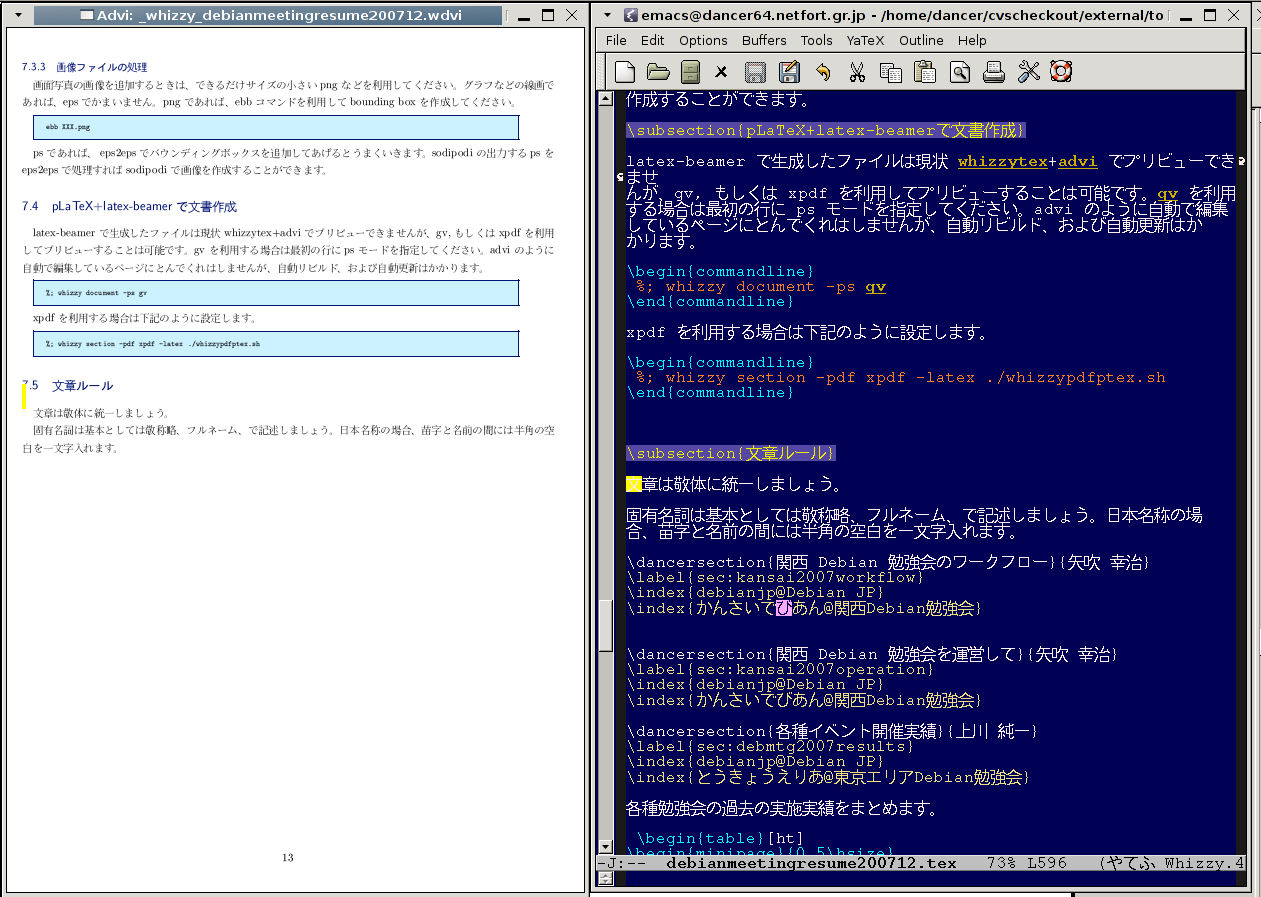
\includegraphics[width=1\hsize]{image200712/whizzytex.png}

\printindex

\cleartooddpage

\vspace*{15cm}
\hrule
\vspace{2mm}

\includegraphics[width=2cm]{image200502/openlogo-nd.eps}
\noindent \Large \bf Debian 勉強会資料\\
\noindent \normalfont \debmtgyear{}年\debmtgmonth{}月\debmtgdate{}日 \hspace{5mm}  初版第1刷発行\\
\noindent \normalfont 東京エリア Debian 勉強会 (編集・印刷・発行)\\
\hrule

\end{document}
